\input{settings}
\setlength{\emergencystretch}{2em}
\titleformat{\section}
  {\small\bfseries\raggedright}
  {}{0em}
  {}
  [{\color{WHU_Blue}\titlerule}]
\titlespacing*{\section}{0cm}{0.85em}{0.60em}
\titlespacing*{\subsection}{0cm}{0.50em}{0.30em}
\setlist[itemize]{topsep=0.20em, itemsep=0.20em, parsep=0em, partopsep=0em, leftmargin=1.25em}
\setlist[enumerate]{topsep=0.20em, itemsep=0.20em, parsep=0em, partopsep=0em, leftmargin=1.35em}
\renewcommand{\arraystretch}{0.98}
\renewcommand{\CJKglue}{\hskip 0.018em}

% 个人信息
%  cd C:\Users\31087\Documents\Obsidian_Vault\Resume\template
%  xelatex main_dataengine.tex
\newcommand{\school}{江南大学 · 控制科学与工程}

\newcommand{\resumeDecor}{
    \begin{tikzpicture}[remember picture, overlay]
        \node[anchor=north, inner sep=0pt](header) at (current page.north){
            
\includegraphics[width=\paperwidth]{images/header.png}
        };
        \node[anchor=west](school_logo) at (header.west){
            \hspace{0.5cm}
            
\includegraphics[width=0.15\textwidth]{images/whu_logo_1.png}
        };
        \node[anchor=east](school_name) at(header.east){
            \textcolor{white}{\textbf{\school}}
            \hspace{0.5cm}
        };
    \end{tikzpicture}

    \begin{tikzpicture}[remember picture, overlay]
        \node[opacity=0.05] at(current page.center){
            
\includegraphics[width=0.68\paperwidth, keepaspectratio]{images/whu_logo_big.png}
        };
    \end{tikzpicture}
}

\newcommand{\sectionIcon}[2]{\makebox[\widthof{#1}][c]{\color{WHU_Blue}{#1}}\quad #2}

%%%%%%%%%%%%%%%%%%%%
% 简历正文
%%%%%%%%%%%%%%%%%%%%
\begin{document}
\resumeDecor
\vspace*{-3.15em}
\scriptsize
\linespread{1.10}\selectfont

% 个人信息
\begin{minipage}{0.80\textwidth}
    \section[个人信息]{\sectionIcon{\faAddressCard}{个人信息}}
    \footnotesize
    \begin{tabularx}{\linewidth}{p{\widthof{求职意向:}}Xp{\widthof{最高学历:}}X}
        姓\ \ \ \ \ \ \ \ 名: & 梁邦一 &
        性\ \ \ \ \ \ \ \ 别: & 男 \\
        邮\ \ \ \ \ \ \ \ 箱: & yuejinai55@gmail.com &
        电\ \ \ \ \ \ \ \ 话: & +86 15515602693 \\
        英语等级: & CET-6 &
        求职意向: & 自动驾驶数据引擎工程师（无锡） \\
    \end{tabularx}
\end{minipage}
\hfill
\begin{minipage}{0.11\textwidth}
    \vspace{2.0em}
    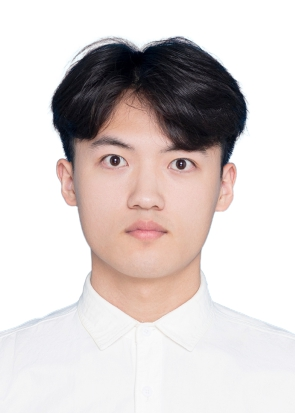
\includegraphics[width=\linewidth]{images/avatar.png}
\end{minipage}
\vspace{-0.60em}

\section[教育背景]{\sectionIcon{\faGraduationCap}{教育背景}}
\begin{itemize}
    \item {\textbf{控制科学与工程硕士，江南大学}}（\hl{中国科学院沈阳自动化研究所 · 机器人与智能系统全国重点实验室联合培养}） \hfill {2024.06--2027.06}
    \item {\textbf{自动化学士，郑州轻工业大学}} \hfill {2020.09--2024.06}
\end{itemize}

% 专业技能
\section[专业技能]{\sectionIcon{\faWrench}{专业技能}}
\begin{itemize}
    \item \textbf{视觉与多模态：}目标检测（YOLO,Gdino）、实例分割（SAM3）、图像分类（Qwen3-VL）、视觉 Embedding 检索(Qwen3-embedding)。
    \item \textbf{推理部署：}ONNX、TensorRT、vllm、SGLang、NVIDIA Jetson AGX Orin，模型量化与端侧推理优化。
    \item \textbf{数据挖掘与自动标注：}规则 Tagger 设计、文搜 + VLM 组合打标、视觉 Embedding 相似检索、伪标签蒸馏、Corner Case 挖掘、标签验收与质量回归。
    \item \textbf{工程能力：}PyTorch、Transformer、Python、C++、LLaMA-Factory（LoRA / 全参数 SFT）、Linux、Git、Docker、ROS2。
\end{itemize}

    % 实习经历
\section[实习经历]{\sectionIcon{\faBriefcase}{实习经历}}
{\small\textbf{CARIZON（大众×地平线合资智驾）}}\quad 感知数据部门算法实习生 \hfill {2026.06--至今}\\
{\scriptsize\color{WHU_Blue} 自动标注工具链 / 数据挖掘与标签质量体系 / VLM 后训练与训练基础设施}
\begin{itemize}
    \item \textbf{感知数据挖掘与标签交付：}面向感知模型训练、评测与地图团队的迭代数据需求，针对复杂场景、长尾场景与 Corner Case 样本获取难、覆盖不足的问题，基于 Qwen3-VL、以图搜图、多源 PB（protobuf）信号构建多模态挖掘方案，形成\hl{“场景挖掘 $\rightarrow$ 复核 $\rightarrow$ 标签交付”的可复用流程}；
    \item \textbf{以图搜图 2.0 方案设计与落地：}针对传统挖掘依赖模型实时推理、成本高且启动慢的问题，参与设计并落地基于视觉相似性的「以图搜图 2.0」——以相似性召回 + 正负例精排完成场景召回与标签生产，不依赖检测 / 分割等额外模型，显著降低数据建设对模型推理资源的依赖；累计交付 \hl{20+ 感知标签}，覆盖蹲着的行人、地面积水中的车辆倒影、行驶区域垃圾袋等高价值 Corner Case，单标签样本通常 >1.5 万，\hl{整体标签准确率超 80\%、人效稳定在 2 个标签 / 人 / 天}。
    \item \textbf{VLM 后训练与标注平台：}围绕闸机杆 / 限高杆多分类任务，完成数据清洗、标注校验与 Prompt 迭代，在 LLaMA-Factory 上完成 \hl{13 轮 SFT 实验迭代}（LoRA $\rightarrow$ 全参、模型蒸馏 CoT），在 \hl{4 机 8 卡 H20 集群}完成全参数 SFT，\hl{测试集准确率 0.8984 创历史新高}；并在 GT 生产平台落地 CoT 标注工具链，形成“人工标注 $\rightarrow$ SFT 训练数据”闭环。
\end{itemize}

\vspace{0.30em}
{\small\textbf{优奇智能科技有限公司（优必选子公司）}}\quad 人形机器人感知算法实习生 \hfill {2026.02--2026.05} \\
{\scriptsize\color{WHU_Blue} 数据质检与标注管理 / Bad Case 归因闭环 / Jetson AGX Orin 端侧部署}
\begin{itemize}
    \item \textbf{数据质检与 Bad Case 归因：}负责多场景视觉数据清洗、类别一致性检查与标注质检，完成训练 / 验证 / 测试集划分；针对误检、漏检及分割边界异常样本，从数据覆盖、标注质量、模型能力等维度归因并制定定向补数方案，形成\hl{“模型评估 $\rightarrow$ Bad Case 归因 $\rightarrow$ 数据改进”的迭代闭环}。
    \item \textbf{端侧部署与推理加速：}负责 R11 接待机器人感知模型在 NVIDIA Jetson AGX Orin 上的端侧部署，完成 PyTorch $\rightarrow$ ONNX $\rightarrow$ TensorRT 模型转换、量化与算子性能优化，\hl{推理延迟降低 20\%}，并在真机跑通检测与分割实时推理链路。
\end{itemize}

\vspace{0.04em}
\section[科研与项目经历]{\sectionIcon{\faFlask}{科研与项目经历}}
{\small\textbf{面向具身智能灵巧操作的肌电-力融合感知与灵巧手抓取控制系统（灵心巧手）} \hfill {2025.02--2026.02} \\
{\scriptsize\color{WHU_Blue} 多模态数据系统 / Transformer 与 Conformer 时序建模 / ROS2 与 MuJoCo 仿真}
\begin{itemize}
    \item \textbf{多模态数据系统：}面向 Linker Hand G20 灵巧手，搭建视觉、sEMG、力 / 触觉及 MuJoCo 仿真的\hl{多模态实验系统}，完成 Delsys Trigno、Sensel 等多通道传感器高频同步采集、时间戳对齐、任务标注与实时可视化，形成可复现的数据入口。
    \item \textbf{时序感知建模：}基于 PyTorch 开展 Transformer / 轻量 Conformer 时序建模，实现肌电信号到指尖力的建模，支持\hl{力等级分类与连续力值回归双任务}；相关 sEMG-Conformer 研究在 Biomedical Signal Processing and Control 在修。
    \item \textbf{系统集成与仿真：}基于 ROS2 构建视觉—仿真策略—sEMG—触觉的模块化感知控制链路，打通 MuJoCo 仿真与真机联调，构成 \hl{Sim-to-Real 端到端方案雏形}，可迁移至多传感器融合感知的数据生产与验证。
\end{itemize}

\section[论文与研究成果]{\sectionIcon{\faBook}{论文与研究成果}}
\begin{itemize}
    \item \hl{已录用 · 第一作者}（JCR 一区 / 中科院二区）：Sensing Technologies for Hand Gesture Recognition in Human-Robot Interaction: A Review. IEEE Sensors Journal, 2025, 26(2): 1501-1519. 
    \item \hl{In Revision（在修）}（JCR 一区 / 中科院二区 Top）：sEMG Conformer: Synergizing Local-Global Spatiotemporal Features for Continuous Force Estimation. Biomedical Signal Processing and Control. 
    \item \hl{Under Review（在投）}（JCR 一区 / 中科院二区）：Dexterous Hand Grasping Control Based on Multimodal Sensory Fusion and Simulation Reinforcement Learning. 
\end{itemize}


% 荣誉与综合素质
\section[荣誉与综合素质]{\sectionIcon{\faStar}{荣誉与综合素质}}
\begin{itemize}
    \item 荣誉奖励：中国机器人大赛暨 RoboCup 机器人世界杯中国赛 \hl{国家三等奖}｜校一等奖学金（2025、2026）｜优秀毕业生。
    \item 组织经历：本科期间曾任班长，硕士期间担任党支部书记。
\end{itemize}

\end{document}
